\documentclass[11pt,UTF8]{ctexart}

\usepackage[margin=2cm,a4paper]{geometry}
%\usepackage[left=0.75in,top=0.6in,right=0.75in,bottom=1.0in,a4paper]{geometry}


\setmainfont{Caladea}
%% 也可以選用其它字庫:
% \setCJKmainfont[%
%   ItalicFont=AR PL KaitiM GB,
%   BoldFont=Noto Sans CJK SC,
% ]{Noto Serif CJK SC}
% \setCJKsansfont{Noto Sans CJK SC}
% \renewcommand{\kaishu}{\CJKfontspec{AR PL KaitiM GB}}

% 繁體中文
\setCJKmainfont[Path=fonts/ ]{NotoSansTC-Medium.otf}


\usepackage{minted}
\usepackage[breaklinks]{hyperref}

% Picture
% 導言區的此三行無變化
\usepackage{graphicx}
\usepackage{float} 
\usepackage{subfigure}
% 以下是新增的自定義格式更改
\usepackage[]{caption2} %新增調用的宏包
\renewcommand{\figurename}{Fig.} %重定義編號前綴詞
\renewcommand{\captionlabeldelim}{.~} %重定義分隔符
 %\roman 是羅馬數字編號,\alph是默認的字母編號,\arabic是阿拉伯數字編號,可按需替換下一行的相應位置
\renewcommand{\thesubfigure}{(\roman{subfigure})}%此外,還可設置圖編號顯示格式,加括號或者不加括號
\makeatletter \renewcommand{\@thesubfigure}{\thesubfigure \space}%子圖編號與名稱的間隔設置
\renewcommand{\p@subfigure}{} \makeatother

% Math
\usepackage {mathtools}
\usepackage{amssymb}

% Code
\usepackage{listings}
\usepackage{xcolor}
\lstset{
    % backgroundcolor=\color{red!50!green!50!blue!50},
    % 程式碼塊背景色為淺灰色
    rulesepcolor= \color{gray}, % 程式碼塊邊框顏色
    breaklines=true,  % 程式碼過長則換行
    numbers=left, % 行號在左側顯示
    numberstyle= \small,% 行號字型
    % eywordstyle= \color{red,% 關鍵字顏色
    commentstyle=\color{gray}, % 註釋顏色
    frame=shadowbox % 用方框框住程式碼塊
    }

\usepackage{hyperref}

\title{數位訊號處理作業}
\author{干皓丞,2101212850, 信息工程學院}

\begin{document}
\maketitle


\section{作業目標}

證明 E3 調整定理

\section{數學說明}

E1, E2 和 E3 之間的關係描述如下,從數學式 (1.1) 的解釋為從 n 次 E3 調整後跟一次E1調整,等價於 1 次 E1 調整後跟 n 次 E2 調整,而數學式 (1.2) 的意義為 n 次 E3 調整後跟一次 E2 調整,等價於 1 次 E2 調整後跟 n 次 E1 調整。
\newline
$$E_{1} \circ (E_{3})^n = (E_{2})^n \circ E_{1} \quad \ (1.1) $$
$$E_{2} \circ (E_{3})^n = (E_{1})^n \circ E_{2} \quad \ (1.2) $$

$E_{i} \circ (E_{j})^n$ : $ n (E_{j})$ scalings, followed by an $E_{i}$ scalling.

\begin{figure}[H]
\centering 
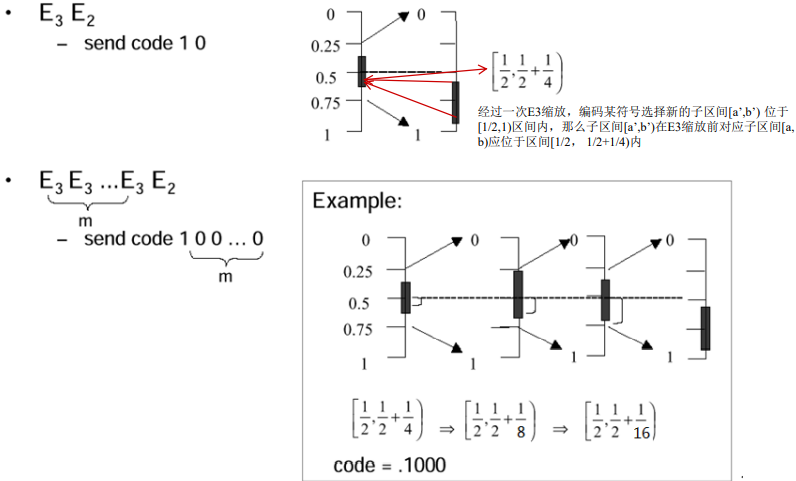
\includegraphics[width=0.95\textwidth]{gp1.png} 
\caption{E3 後面跟 E2}
\label{Test}
\end{figure}

\begin{figure}[H]
\centering 
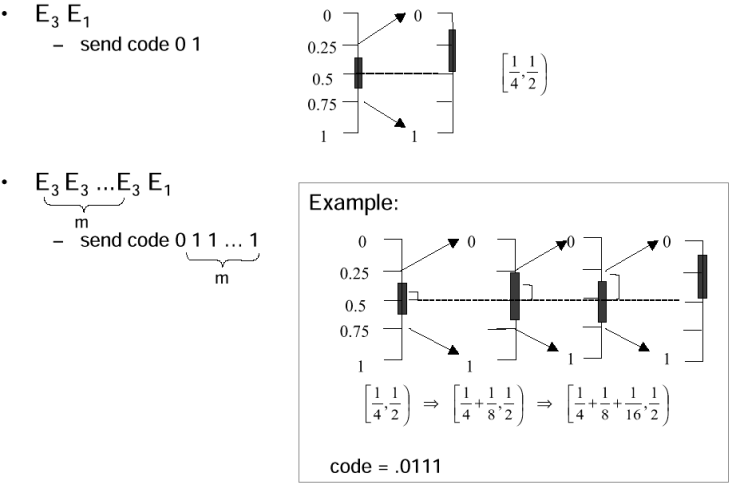
\includegraphics[width=0.95\textwidth]{gp2.png} 
\caption{E3 後面跟 E1}
\label{Test}
\end{figure}

\section{E3 調整定理證明}

在此設 f 和 g 是兩個函數,$ g \circ f $ 是 f 和 g 的連續應用 (the consecutive application)。那麼我們可以將方法表達如下:

LEMMA  適用於任何序列,以下等式都是有效的,下面為之前的數學式 (1.1) 和 (1.2):

$$E_{1} \circ (E_{3})^n = (E_{2})^n \circ E_{1} \quad \ (1.1) $$

$$E_{2} \circ (E_{3})^n = (E_{1})^n \circ E_{2} \quad \ (1.2) $$

證明:

讓 a := low, b := high 和 I := [0,1) 是我們正在使用的間隔,其縮放函數 (The scaling functions) 可以表示如下:

$$E_1\left(\begin{matrix}a\\b\\\end{matrix}\right)=\left(\begin{matrix}2a\\2b\\\end{matrix}\right) \quad \ (3.1)$$

$$E_2\left(\begin{matrix}a\\b\\\end{matrix}\right)=\left(\begin{matrix}2a-1\\2b-1\\\end{matrix}\right) \quad \ (3.2) $$

$$E_3\left(\begin{matrix}a\\b\\\end{matrix}\right)=\left(\begin{matrix}2a-\frac{1}{2}\\2b-\frac{1}{2}\\\end{matrix}\right) \quad \ (3.3) $$

第 n 次迭代結果

$$E_1^n\left(\begin{matrix}a\\b\\\end{matrix}\right)=\left(\begin{matrix}2^na\\2^nb\\\end{matrix}\right) \quad \ (3.4) $$

$$E_2^n\left(\begin{matrix}a\\b\\\end{matrix}\right)=\left(\begin{matrix}2^na-2^n+1\\2^nb-2^n+1\\\end{matrix}\right) \quad \ (3.5) $$

$$E_3^n\left(\begin{matrix}a\\b\\\end{matrix}\right)=\left(\begin{matrix}2^na-2^{n-1}+\frac{1}{2}\\2^nb-2^{n-1}+\frac{1}{2}\\\end{matrix}\right) \quad \ (3.6) $$

歸納證明後,得出以下兩個數學式:

$$(E_1 \circ {(E_3)}^n)\left(\begin{matrix}a\\b\\\end{matrix}\right)=E_1\left(\begin{matrix}2^na-2^{n-1}+\frac{1}{2}\\2^nb-2^{n-1}+\frac{1}{2}\\\end{matrix}\right)=\left(\begin{matrix}2^{n+1}a-2^n+ 1 \\2^{n+1}b-2^n+ 1 \\\end{matrix}\right) \quad \ (3.7) $$

$$({(E_2)}^n \circ E_1)\left(\begin{matrix}a\\b\\\end{matrix}\right)={(E_2)}^n\left(\begin{matrix}2a\\2b\\\end{matrix}\right)=\left(\begin{matrix}2^{n+1}a-2^n+1\\2^{n+1}b-2^n+1\\\end{matrix}\right) \quad \ (3.8) $$

數學式 (3.7) 和 (3.8) ,即為原本的數學式 (1.1) :

$$E_{1} \circ (E_{3})^n = (E_{2})^n \circ E_{1} \quad \ (1.1) $$

反之亦然可以用類似的方式證明數學式 (1.2)。

$$(E_2 \circ {(E_3)}^n)\left(\begin{matrix}a\\b\\\end{matrix}\right)=E_2\left(\begin{matrix}2^na-2^{n-1}+\frac{1}{2}\\2^nb-2^{n-1}+\frac{1}{2}\\\end{matrix}\right)=\left(\begin{matrix}2^{n+1}a-2^n\\2^{n+1}b-2^n\\\end{matrix}\right) \quad \ (3.9) $$

$$({(E_2)}^n \circ E_1)\left(\begin{matrix}a\\b\\\end{matrix}\right)={(E_1)}^n\left(\begin{matrix}2a-1\\2b-1\\\end{matrix}\right)=\left(\begin{matrix}2^{n+1}a-2^n\\2^{n+1}b-2^n\\\end{matrix}\right) \quad \ (3.10) $$

\clearpage

\end{document}